\documentclass[11pt]{beamer}
\usetheme{Madrid}
\usepackage[utf8]{inputenc}

\usepackage{hyperref}
\usepackage{amsmath}
\usepackage{amsfonts}
\usepackage{amssymb}
\usepackage{graphicx}
\usepackage{algorithmic}
\usepackage{algorithm}
\usepackage{wrapfig}
\usepackage{subcaption}
\graphicspath{{.}}

\author{Hongda Li}
\title[Catalyst Acceleration]{Catalyst Meta Acceleration Framework: The history and the gist of it}
% Informe o seu email de contato no comando a seguir
% Por exemplo, alcebiades.col@ufes.br
\newcommand{\email}{alto@mail.ubc.ca}
\setbeamercovered{transparent}
\setbeamertemplate{navigation symbols}{}
%\logo{}
\institute[]{UBC Okanagan}
\date{\today}
\subject{MATH 590 2024 Fall Winter}

% ---------------------------------------------------------
% Selecione um estilo de referência
\bibliographystyle{IEEEtran}

%\bibliographystyle{abbrv}
%\setbeamertemplate{bibliography item}{\insertbiblabel}
% ---------------------------------------------------------

% ---------------------------------------------------------
\newtheorem{remark}{Remark}
\newtheorem{assumption}{Assumption}


% These are Heniz's notations. 
\newcommand{\To}{\ensuremath{\rightrightarrows}}
\newcommand{\GX}{\ensuremath{\Gamma}}
\newcommand{\mal}{\ensuremath{\mathfrak{m}}}
\newcommand{\mumu}{\ensuremath{{\mu\mu}}}
\newcommand{\paver}{\ensuremath{\mathcal{P}}}
\newcommand{\ZZZ}{\ensuremath{{X \times X^*}}}
\newcommand{\RRR}{\ensuremath{{\RR \times \RR}}}
\newcommand{\todo}{\hookrightarrow\textsf{TO DO:}}

\newcommand{\emp}{\ensuremath{\varnothing}}
%\newcommand{\la}{\ensuremath{\langle}}
%\newcommand{\ra}{\ensuremath{\rangle}}
\newcommand{\infconv}{\ensuremath{\mbox{\small$\,\square\,$}}}
\newcommand{\pscal}{\ensuremath{\scal{\cdot}{\cdot}}}
\newcommand{\Tt}{\ensuremath{\mathfrak{T}}}
\newcommand{\YY}{\ensuremath{\mathcal Y}}
\newcommand{\XX}{\ensuremath{\mathcal X}}
\newcommand{\HH}{\ensuremath{\mathcal H}}
\newcommand{\XP}{\ensuremath{\mathcal X}^*}
\newcommand{\st}{\ensuremath{\;|\;}}
\newcommand{\zeroun}{\ensuremath{\left]0,1\right[}}

\newcommand{\lev}[1]{\ensuremath{\mathrm{lev}_{\leq #1}\:}}
\newcommand{\moyo}[2]{\ensuremath{\sideset{_{#2}}{}{\operatorname{}}\!#1}}
\newcommand{\pair}[2]{\left\langle{{#1},{#2}}\right\rangle}
%\newcommand{\scal}[2]{\left.\left\langle{#1}\:\right| {#2}  \right\rangle}
\newcommand{\scal}[2]{\langle{{#1},{#2}}\rangle}
\newcommand{\Scal}[2]{\left\langle{{#1},{#2}}\right\rangle}
%\newcommand{\scal}[2]{\braket{ {#1},{#2}}}

\newcommand{\yosida}{\ensuremath{ \; {}^}}
\newcommand{\exi}{\ensuremath{\exists\,}}
\newcommand{\GG}{\ensuremath{\mathcal G}}
\newcommand{\RR}{\ensuremath{\mathbb R}}
\newcommand{\SSS}{\ensuremath{\mathbb S}}
\newcommand{\CC}{\ensuremath{\mathbb C}}
\newcommand{\Real}{\ensuremath{\mathrm{Re}\,}}
\newcommand{\ii}{\ensuremath{\mathrm i}}
\newcommand{\RP}{\ensuremath{\left[0,+\infty\right[}}
\newcommand{\RPX}{\ensuremath{\left[0,+\infty\right]}}
\newcommand{\RPP}{\ensuremath{\,\left]0,+\infty\right[}}
\newcommand{\RX}{\ensuremath{\,\left]-\infty,+\infty\right]}}
\newcommand{\RXX}{\ensuremath{\,\left[-\infty,+\infty\right]}}
\newcommand{\KK}{\ensuremath{\mathbb K}}
\newcommand{\NN}{\ensuremath{\mathbb N}}
\newcommand{\nnn}{\ensuremath{{n \in \NN}}}
\newcommand{\thalb}{\ensuremath{\tfrac{1}{2}}}
\newcommand{\zo}{\ensuremath{{\left]0,1\right]}}}
\newcommand{\lzo}{\ensuremath{{\lambda \in \left]0,1\right]}}}
%\newcommand{\toppsepp}{\setlength{\partopsep}{-5pt}}
\newcommand{\menge}[2]{\big\{{#1} \mid {#2}\big\}}
\newcommand{\pfrac}[2]{\ensuremath{\mathlarger{\tfrac{#1}{#2}}}}


% MATH OPERATORS ===============================================================
% \newcommand{\monos}{\ensuremath{\mathcal M}}
\newcommand{\DD}{\operatorname{dom}f}
\newcommand{\IDD}{\ensuremath{\operatorname{int}\operatorname{dom}f}}
\newcommand{\CDD}{\ensuremath{\overline{\operatorname{dom}}\,f}}
\newcommand{\clspan}{\ensuremath{\overline{\operatorname{span}}}}
\newcommand{\cone}{\ensuremath{\operatorname{cone}}}
\newcommand{\dom}{\ensuremath{\operatorname{dom}}}
\newcommand{\closu}{\ensuremath{\operatorname{cl}}}
\newcommand{\cont}{\ensuremath{\operatorname{cont}}}
\newcommand{\mons}{\ensuremath{\mathcal{A}}}
\newcommand{\gra}{\ensuremath{\operatorname{gra}}}
\newcommand{\epi}{\ensuremath{\operatorname{epi}}}
\newcommand{\prox}{\ensuremath{\operatorname{Prox}_{\mu}}}
\newcommand{\hprox}{\ensuremath{\operatorname{prox}}}
\newcommand{\intdom}{\ensuremath{\operatorname{int}\operatorname{dom}}\,}
\newcommand{\inte}{\ensuremath{\operatorname{int}}}
\newcommand{\sri}{\ensuremath{\operatorname{sri}}}
\newcommand{\reli}{\ensuremath{\operatorname{ri}}}
\newcommand{\cart}{\ensuremath{\mbox{\LARGE{$\times$}}}}


\newcommand{\average}{\ensuremath{\mathcal{R}_{\mu}({\bf A},{\boldsymbol \lambda})}}
\newcommand{\averagebar}{\ensuremath{\mathcal{R}_{1}({\bf A},\bar{\lambda})}}
\newcommand{\averageonelambda}{\ensuremath{\mathcal{R}({\bf A},{\boldsymbol \lambda})}}
\newcommand{\averageonehalf}{\ensuremath{\mathcal{R}_{1}(A,1/2)}}
\newcommand{\averageinverse}{\ensuremath{\mathcal{R}_{\mu^{-1}}({\bf A}^{-1},{\boldsymbol \lambda})}}
\newcommand{\averageoneinverse}{\ensuremath{\mathcal{R}({\bf A}^{-1},{\boldsymbol \lambda})}}
\newcommand{\averagef}{\ensuremath{\mathcal{P}_{\mu}(f,\lambda)}}
\newcommand{\averagefone}{\ensuremath{\mathcal{P}_{1}(f,\lambda)}}
\newcommand{\averagefd}{\ensuremath{\mathcal{P}_{\mu}((f_{1},\ldots, f_{n}),(\lambda_{1},\ldots, \lambda_{n}))}}
\newcommand{\averagefik}{\ensuremath{\mathcal{P}_{\mu_{k}}((f_{1,k},\ldots,f_{n,k}),
(\lambda_{1,k},\ldots,\lambda_{n,k}))}}
\newcommand{\averagesub}{\ensuremath{\mathcal{R}_{\mu}(\partial f,\lambda)}}
\newcommand{\res}{\ensuremath{\mathcal{R}_{\mu}}}
\newcommand{\resmuk}{\ensuremath{\mathcal{R}_{\mu_{k}}}}
\newcommand{\newres}{\ensuremath{\mathcal{R}}}
\newcommand{\resmualpha}{\ensuremath{\mathcal{R}_{\alpha\mu}}}
\newcommand{\averageone}{\ensuremath{\mathcal{R}_{1}}}
\newcommand{\harm}{\ensuremath{\mathcal{H}(A,\lambda)}}
\newcommand{\arithmetic}{\ensuremath{\mathcal{A}(A,\lambda)}}

\newcommand{\WC}{\ensuremath{{\mathfrak W}}}
\newcommand{\SC}{\ensuremath{{\mathfrak S}}}
\newcommand{\card}{\ensuremath{\operatorname{card}}}
\newcommand{\bd}{\ensuremath{\operatorname{bdry}}}
\newcommand{\ran}{\ensuremath{\operatorname{ran}}}
\newcommand{\rec}{\ensuremath{\operatorname{rec}}}
\newcommand{\rank}{\ensuremath{\operatorname{rank}}}
\newcommand{\kernel}{\ensuremath{\operatorname{ker}}}
\newcommand{\conv}{\ensuremath{\operatorname{conv}}}
\newcommand{\segh}{\ensuremath{\operatorname{seg}}}
\newcommand{\boxx}{\ensuremath{\operatorname{box}}}
\newcommand{\clconv}{\ensuremath{\overline{\operatorname{conv}}\,}}
\newcommand{\cldom}{\ensuremath{\overline{\operatorname{dom}}\,}}
\newcommand{\clran}{\ensuremath{\overline{\operatorname{ran}}\,}}
\newcommand{\Nf}{\ensuremath{\nabla f}}
\newcommand{\NNf}{\ensuremath{\nabla^2f}}
\newcommand{\Fix}{\ensuremath{\operatorname{Fix}}}
\newcommand{\FFix}{\ensuremath{\overline{\operatorname{Fix}}\,}}
\newcommand{\aFix}{\ensuremath{\widetilde{\operatorname{Fix}\,}}}
\newcommand{\Id}{\ensuremath{\operatorname{Id}}}
\newcommand{\Max}{\ensuremath{\operatorname{max}}}
\newcommand{\Bb}{\ensuremath{\mathfrak{B}}}
\newcommand{\BB}{\ensuremath{\mathbb{B}}}
\newcommand{\Fb}{\ensuremath{\overrightarrow{\mathfrak{B}}}}
\newcommand{\Fprox}{\ensuremath{\overrightarrow{\operatorname{prox}}}}
\newcommand{\Bprox}{\ensuremath{\overleftarrow{\operatorname{prox}}}}
\newcommand{\Bproj}{\ensuremath{\overleftarrow{\operatorname{P}}}}
\newcommand{\Ri}{\ensuremath{\mathfrak{R}_i}}
\newcommand{\Dn}{\ensuremath{\,\overset{D}{\rightarrow}\,}}
\newcommand{\nDn}{\ensuremath{\,\overset{D}{\not\rightarrow}\,}}
\newcommand{\weakly}{\ensuremath{\,\rightharpoonup}\,}
\newcommand{\weaklys}{\ensuremath{\,\overset{*}{\rightharpoonup}}\,}
\newcommand{\gr}{\ensuremath{\operatorname{gra}}}
\newcommand{\g}{\ensuremath{\,\overset{g}{\rightarrow}}\,}
\newcommand{\p}{\ensuremath{\,\overset{p}{\rightarrow}}\,}
\newcommand{\e}{\ensuremath{\,\overset{e}{\rightarrow}}\,}
\newcommand{\Tbar}{\ensuremath{\overline{T}}}
\newcommand{\n}{\ensuremath{\,\overset{n}{\rightarrow}}\,}

\newcommand{\minf}{\ensuremath{-\infty}}
\newcommand{\pinf}{\ensuremath{+\infty}}
\renewcommand{\iff}{\ensuremath{\Leftrightarrow}}
% \renewcommand{\phi}{\ensuremath{\varphi}}
%\newcommand{\Real}{\ensuremath{\mathrm{Re}\,}}
\newcommand{\negent}{\ensuremath{\operatorname{negent}}}
\newcommand{\neglog}{\ensuremath{\operatorname{neglog}}}
\newcommand{\halb}{\ensuremath{\tfrac{1}{2}}}
\newcommand{\bT}{\ensuremath{\mathbf{T}}}
\newcommand{\bX}{\ensuremath{\mathbf{X}}}
\newcommand{\bL}{\ensuremath{\mathbf{L}}}
\newcommand{\bD}{\ensuremath{\boldsymbol{\Delta}}}
\newcommand{\bc}{\ensuremath{\mathbf{c}}}
\newcommand{\by}{\ensuremath{\mathbf{y}}}
\newcommand{\bx}{\ensuremath{\mathbf{x}}}
\newcommand{\bA}{{\bf A}}
\newcommand{\Other}{Indeterminate }
\newcommand{\other}{indeterminate }


%%% Raf's stuff  ===============================================================
\newcommand{\al}{\alpha}
\newcommand{\la}{\lambda}
\newcommand{\La}{\Lambda}
\newcommand{\pluss}{{\hskip1pt \raise1pt\vbox{\hrule width6pt \vskip1pt
\hrule width6pt}\kern-4pt{\lower1pt\hbox{\vrule height6pt \kern1pt\vrule
height6pt}}\hskip5pt}}
\newcommand{\timess}{\star}
\newcommand{\argmax}{\mathop{\rm argmax}\limits}
\newcommand{\argmin}{\mathop{\rm argmin}\limits}
\newcommand{\product}{\langle\cdot,\cdot\rangle}
\newcommand{\im}{\mathrm{Im}}
\newcommand{\multival}{\ensuremath{X\to 2^{X^*}}}
\newcommand{\SX}{\ensuremath{2^{X^*}}}




\begin{document}

\begin{frame}
    \titlepage
\end{frame}

\begin{frame}{ToC}
    \tableofcontents
\end{frame}

%     \subsection{Taxonomy of Proximal type of Methods}
%         \begin{frame}{Frame Title}
    
%             \begin{block}{Formula Presented in Block}
%                 \begin{align}
%                     \min_{x} g(x) + h(x)
%                 \end{align}    
%             \end{block}
            
%             \begin{itemize}
%                 \item [1.]Throughout this presentation, we assume the objective of a function $f$ is the sum of 2 functions.
%                 \item [2.]We are interested in the paper: FISTA (Fast Iterative-Shrinkage Algorithm) by Beck and Teboulle \cite{paper:FISTA}. 
%                 \pause 
%                 \item [1.] When $h = \delta_Q$ with $Q$ closed and convex with $Q\subseteq \text{ri}\circ \text{dom}(g)$, we use projected subgradient. 
%                 \item [2.] When $g$ is \textbf{\emph{strongly smooth}} and $h$ is \textbf{closed convex proper} whose proximal oracle is easy to compute, we consider the use of FISTA. 
%             \end{itemize}
                
%         \end{frame}
        
%     \subsection{The Proximal Operator}
%         \begin{frame}{Frame Title}
%             \begin{definition}[Definition of Something]
%                 Let $f$ be convex closed and proper, then the proximal operator parameterized by $\alpha > 0$ is a non-expansive mapping defined as: 
%                 \begin{align*}
%                     \text{prox}_{f, \alpha}(x) := 
%                     \arg\min_{y}\left\lbrace
%                         f(y) + \frac{1}{2\alpha} \Vert y - x\Vert^2
%                     \right\rbrace. 
%                 \end{align*}
%             \end{definition}  
%             \begin{remark}
%                 When $f$ is convex, closed, and proper, 
%             \end{remark}
%         \end{frame}

%         \begin{frame}{Prox is the Resolvant of Subgradient}
%             \begin{lemma}[The Lemma]\label{lemma:prox_alternative_form}
%                 When the function $f$ is convex closed and proper, the $\text{prox}_{\alpha, f}$ can be viewed as the following operator $(I + \alpha \partial f)^{-1}$. 
%             \end{lemma}
%             \begin{proof}
%                 Minimizer satisfies zero subgradient condition, 
%                 {\scriptsize
%                 \begin{align*}
%                     \mathbf 0 &\in \partial
%                     \left[
%                         \left.
%                             f(y) + \frac{1}{2\alpha} \Vert y - x\Vert^2 
%                         \right| y
%                     \right](y^+)
%                     \\
%                     \mathbf 0 &\in \partial f(y^+) + \frac{1}{\alpha}(y^+ - x)
%                     \\
%                     \frac{x}{\alpha} &\in 
%                     (\partial f + \alpha^{-1}I)(y^+)
%                     \\
%                     x &\in 
%                     (\alpha \partial f + I)(y^+)
%                     \\
%                     y &\in (\alpha\partial f+ I)^{-1}(x).
%                 \end{align*}
%                 }
%             \end{proof}
                
%         \end{frame}
        
        
%     \subsection{Strong Smoothness}
%         \begin{frame}{Equivalence of Strong Smoothness and Lipschitz Gradient}
%             \begin{theorem}[Lipschitz Gradient Equivalence under Convexity]
%                 Suppose $g$ is differentiable on the entire of $\mathbb E$. It is closed convex proper. It is strongly smooth with parameter $\alpha$ if and only if the gradient $\nabla g$ is globally Lipschitz continuous with a parameter of $\alpha$ and $g$ is closed and convex. 
%                 \begin{align*}
%                     \Vert \nabla g(x) -\nabla g(y)\Vert \le 
%                     \alpha 
%                     \Vert x - y \Vert\quad \forall x, y\in \mathbb E
%                 \end{align*}
%             \end{theorem}
%             \begin{proof}
%                 Using line integral, we can prove Lipschitz gradient implies strong smoothness without convexity. The converse requires convexity and applying generalized Cauchy Inequality to (iv) in Theorem 5.8 for Beck's textbook \cite{book:first_order_opt}. 
%             \end{proof}
            
%         \end{frame}
%     \subsection{A Major Assumption}    
%         \begin{frame}{A Major Assumption}
%             \begin{assumption}[Convex Smooth Nonsmooth with Bounded Minimizers]\label{assumption:1}
%                 We will assume that $g:\mathbb E\mapsto \mathbb R$ is \textbf{strongly smooth} with constant $L_g$ and $h:\mathbb E \mapsto \bar{\mathbb R}$ \textbf{is closed convex and proper}. We define $f := g + h$ to be the summed function and $\text{ri}\circ \text{dom}(g) \cap \text{ri}\circ \text{dom}(h) \neq \emptyset$. We also assume that a set of minimizers exists for the function $f$ and that the set is bounded. Denote the minimizer using $\bar x$. 
%             \end{assumption}
%         \end{frame}
        
    
% \section{A New Fancy Section}
%     \subsection{A Fancy Subsetction for Algorithm}
%         \begin{frame}{The Accelerated Proximal Gradient Method}
%             \begin{block}{Momentum Template Method}
%                 \begin{algorithm}[H]
%                     \begin{algorithmic}[1]
%                         \STATE{\textbf{Input:} $x^{(0)}, x^{(-1)}, L, h, g$; 2 initial guesses and stepsize L}
%                         \STATE{$y^{(0)} = x^{(0)} + \theta_k (x^{(0)} - x^{(-1)})$}
%                         \FOR{$k = 1, \cdots, N$}
%                             \STATE{$x^{(k)} = \text{prox}_{h, L^{-1}}(y^{(k)} + L^{-1}\nabla g(y^{(k)})) =: \mathcal P_{L^{-1}}^{g, h}(y^{(k)})$}
%                             \STATE{$y^{(k + 1)} = x^{(k)} + \theta_k(x^{(k)} - x^{(k - 1)})$}
%                         \ENDFOR
%                     \end{algorithmic}
%                     \caption{Template Proximal Gradient Method With Momentum}\label{alg:fista_template}
%                 \end{algorithm}
%             \end{block}
%         \end{frame}

\section{Introduction}
    \subsection{The History and a Series of Papers}
        \begin{frame}{Nesterov's Book}
            \begin{figure}
                \centering
                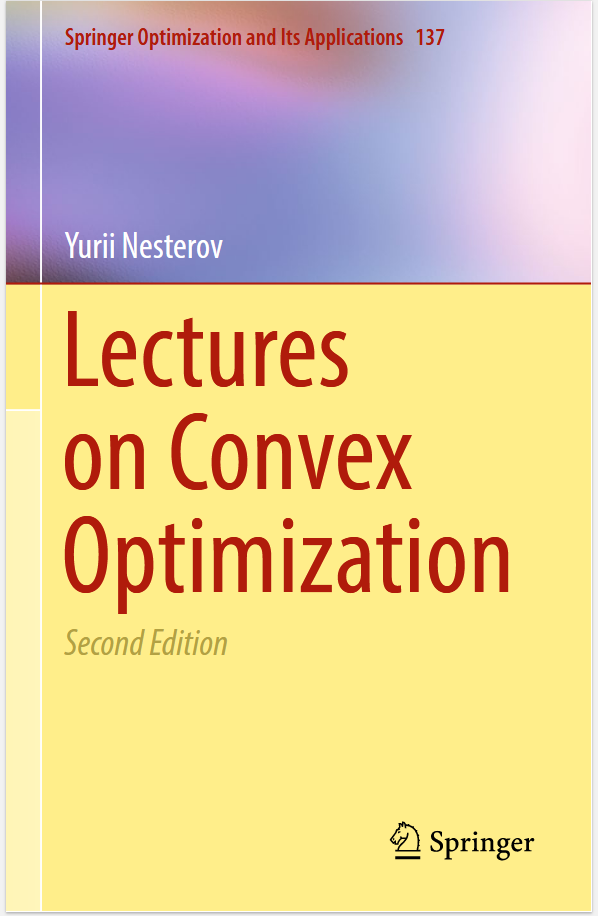
\includegraphics[width=10em]{assets/Nesterov Book.png}    
            \end{figure}
            \begin{itemize}
                \item Yurri Nesterov's book: ``Lectures on Convex Optimization'' 2018, Springer \cite{nesterov_lectures_2018}. 
            \end{itemize}
        \end{frame}
        \begin{frame}{Accelerated Proximal Point Method}
            \begin{figure}
                \centering
                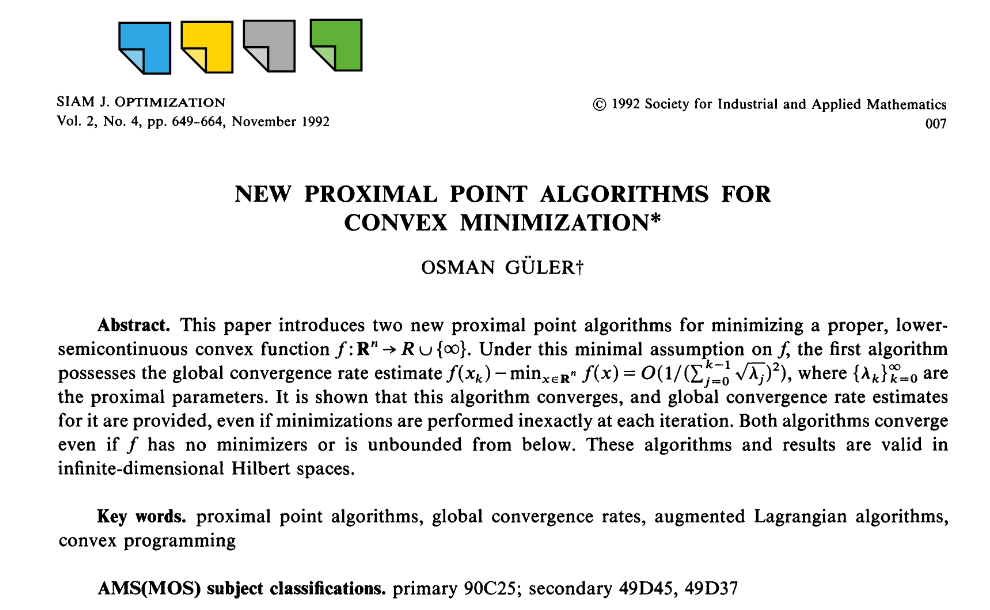
\includegraphics[width=25em]{assets/Acc ppm}
            \end{figure}
            \begin{itemize}
                \item Osman Guler's, ``New proximal point algorithm for convex optimization'', SIAM J.Optimization 1992. \cite{guler_new_1992}
            \end{itemize}
        \end{frame}
        \begin{frame}{Catalyst Acceleration}
            \begin{figure}
                \centering
                \subfloat[Lin 2015\label{fig:a}]{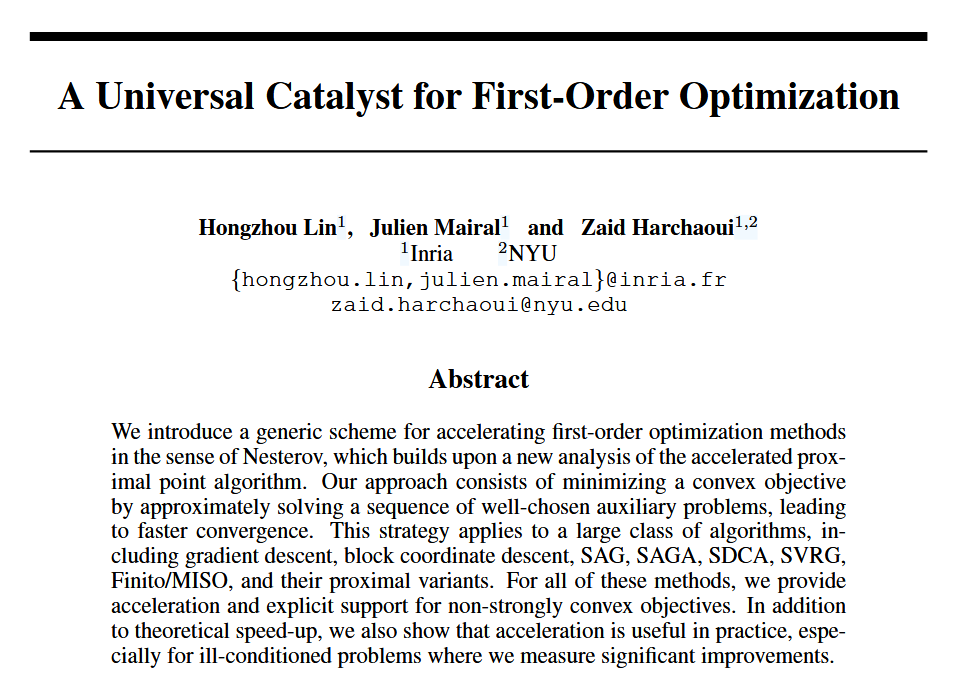
\includegraphics[width=15em]{assets/lin2015.png}}
                \subfloat[Paquette 2018\label{fig:b}]{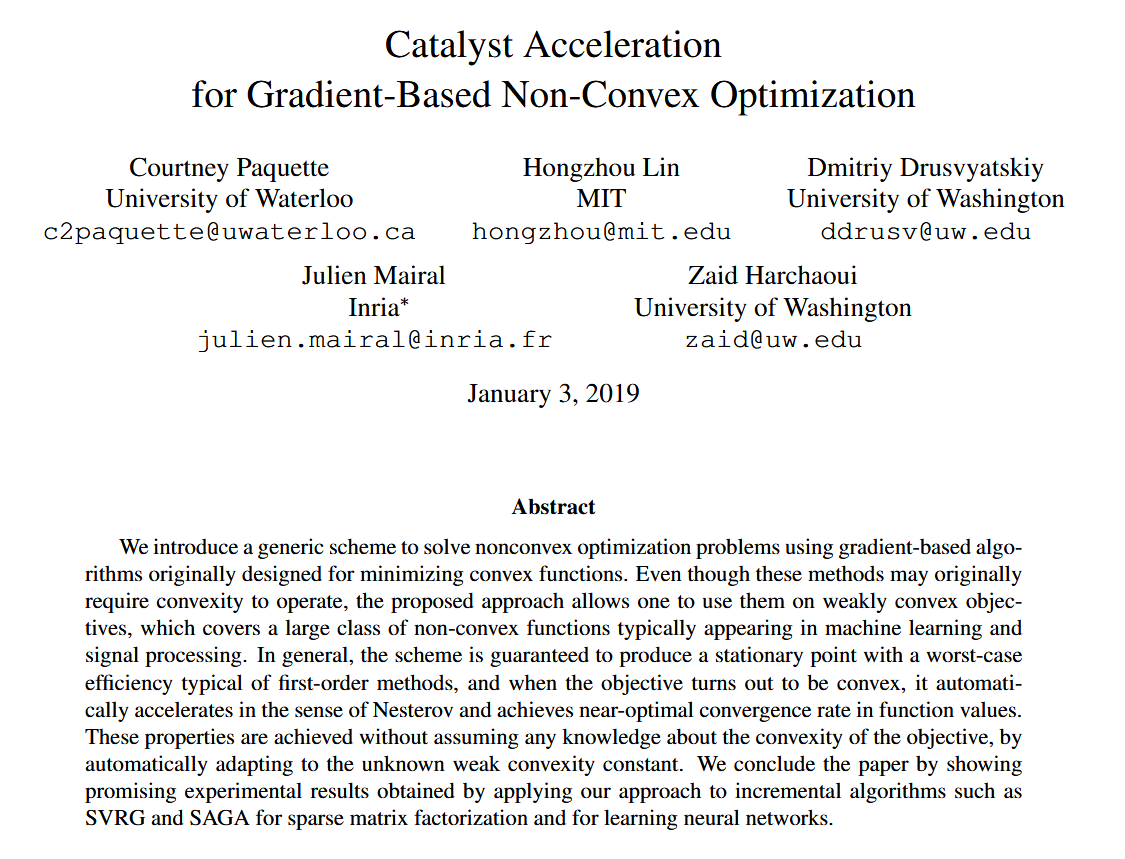
\includegraphics[width=15em]{assets/paquette 2018.png}}
                % \caption{Lin's }
                % \label{fig:1}
            \end{figure}
            \begin{itemize}
                \item Honzhou Lin et al. ``Universal Catalyst for first order optimization'' 2015 JLMR \cite{lin_universal_2015}.
                \item Paquette et al. ``Catalyst for gradient-based nonconvex optimization'' 2018 JLMR \cite{paquette_catalyst_2018}. 
            \end{itemize}
        \end{frame}
        \begin{frame}{Objectives of the Talk}
            \begin{block}{List of objectives}
                \begin{enumerate}
                    \item Introduce the technique of Nesterov's estimating sequence for convergence proof of algorithms. 
                    \item Understand the historical context for the inspirations of the Catalyst algorithm.  
                    \item Understand the theories behind the Catalyst meta acceleration. 
                    \item Understand key innovations for controlling the errors in Catalyst accelerations. 
                    \item Introduce the Non-convex extension of the method. 
                \end{enumerate}
            \end{block}
            \pause
            \begin{block}{A note on the scope}
                Specific applications and algorithms are outside of the scope because variance reduced stochastic method is itself a big topic.     
            \end{block}
        \end{frame}
        \begin{frame}{Quick Notations}
            
        \end{frame}
    \subsection{Nesterov's Estimating Sequence}
        \begin{frame}{Nesterov's Estimating Sequence}            
            \begin{definition}[Nesterov's estimating sequence]\label{def:nes-est-seq}
                Let $(\phi_k : \RR^n \mapsto \RR)_{k \ge 0}$ be a sequence of functions. 
                We call this sequence of function a Nesterov's estimating sequence when it satisfies the conditions that: 
                \begin{enumerate}
                    \item There exists another sequence $(x_k)_{k \ge 0}$ such that for all $k \ge 0$ it has $F(x_k) \le \phi_k^*$. 
                    \item There exists a sequence of $(\alpha_k)_{k \ge 0}$ such that for all $x \in \RR^n$, $\phi_{k + 1}(x) - \phi_k(x) \le - \alpha_k(\phi_k(x) - F(x))$. 
                \end{enumerate}
            \end{definition}
        \end{frame}

        \begin{frame}{Nesterov's Estimating Sequence and Convergence}
            \begin{block}{Observations}
                {\small
                If we dsefine $\phi_k$, $\Delta_k(x) := \phi_k (x) - F(x)$ for all $x \in \RR^n$ and assume that $F$ has minimizer $x^*$. 
                Then observe that $\forall k \ge 0$:  
                \begin{align*}
                    \phi_{k + 1}(x) - \phi_k(x) 
                    &\le - \alpha_k (\phi_k(x) - F(x))
                    \\
                    \iff 
                    \phi_{k + 1}(x) - F(x) - (\phi_k(x) - F(x))
                    &\le 
                    -\alpha_k(\phi_k(x) - F(x))
                    \\
                    \iff
                    \Delta_{k + 1}(x) - \Delta_k(x) &\le
                    - \alpha_k\Delta_k(x)
                    \\
                    \iff 
                    \Delta_{k + 1}(x) 
                    &\le 
                    (1 - \alpha_k)\Delta_k(x). 
                \end{align*}
                Unroll the recurrence, by setting $x = x^*$, $\Delta_k(x^*)$ is non-negative and using the property of Nesterov's estimating sequence it gives: 
                \begin{align*}
                    F(x_k) - F(x^*) \le \phi_k^* - F(x^*) \le \Delta_k(x^*) 
                    &= \phi_k(x^*) - F(x^*) 
                    \\
                    &\le \left(\prod_{i = 0}^k(1 - \alpha_i)\right)\Delta_0(x^*).
                \end{align*}
                }
            \end{block}
            
        \end{frame}
        \begin{frame}{Example: accelerated proximal gradient}
            \begin{block}{Quick Notations}
                Assume that: $F = f + g$ where $f$ is $L$-Lipschitz smooth and $\mu \ge 0$ strongly convex and $g$ is convex. 
                Define 
                \begin{align*}
                    \mathcal M^{L^{-1}}(x; y) 
                    &:= g(x) + f(y) 
                    + 
                    \left\langle \nabla f(x), x - y\right\rangle 
                    + 
                    \frac{L}{2}\Vert x - y\Vert^2, 
                    \\
                    \widetilde{\mathcal J}_{L^{-1}}y 
                    &:= \argmin_{x} \mathcal M^{L^{-1}}(x; y), 
                    \\
                    \mathcal G_{L^{-1}}(y)
                    &:= L\left(I - \widetilde{\mathcal J}_{L^{-1}}\right)y. 
                \end{align*}

            \end{block}
        \end{frame}

        \begin{frame}{Example: accelerated proximal gradient}
            \begin{definition}[Accelerated proximal gradient estimating sequence]
                \label{def:nes-est-seq-pg}
                {\small
                    Define $(\phi_k)_{k \ge0}$ be the Nesterov's estimating sequence recursively given by: 
                    \begin{align*}
                        & l_F(x; y_k) := 
                            F\left(\widetilde{\mathcal J}_{L^{-1}} y_k \right) 
                            + \langle \mathcal G_{L^{-1}}y_k, x - y_k\rangle + 
                        \frac{1}{2L}\Vert \mathcal G_{L^{-1}}y_k\Vert^2, 
                        \\
                        & 
                        \phi_{k + 1}(x)
                        := (1 - \alpha_k)\phi_k (x) + 
                        \alpha_k 
                        \left(
                            l_F(x; y_k) + \frac{\mu}{2}\Vert x - y_k\Vert^2
                        \right). 
                    \end{align*}
                    The Algorithm generates a sequence of vectors $y_k, x_k$, and scalars $\alpha_k$ satisfies the following: 
                    \begin{align*}
                        &x_{k + 1} = \widetilde{\mathcal J}_{L^{-1}} y_k, 
                        \\
                        & \text{find } \alpha_{k + 1} \in (0, 1): 
                        \alpha_{k + 1} = (1 - \alpha_{k + 1})\alpha_k^{2} + (\mu/L) \alpha_{k + 1}
                        \\
                        &y_{k + 1} = x_{k + 1} + \frac{\alpha_k(1 - \alpha_k)}{\alpha_k^2 + \alpha_{k + 1}}(x_{k + 1} - x_k). 
                    \end{align*}
                    One of the possible base case can be $x_0 = y_0$ and any $\alpha_0 \in (0, 1)$. 
                }
            \end{definition}
                
        \end{frame}

\section{Guler 1993}
\section{Lin 2015}
\section{Paquette 2018}
        
    
\section{References}
    \begin{frame}{References}
        \bibliography{references/refs.bib}
    \end{frame}

\end{document}